\section{Implementierung von Reglern \buchSeite{147}}
Es wird eine \textit{minimale} Implementierung angestrebt, was bedeutet, dass die Anzahl
der Integratoren minimal sein soll. Wenn der gegebene Regler $G_R(s)$ vollständig
gekürzt ist, dann hat eine minimale Implementierung n Integratoren.
%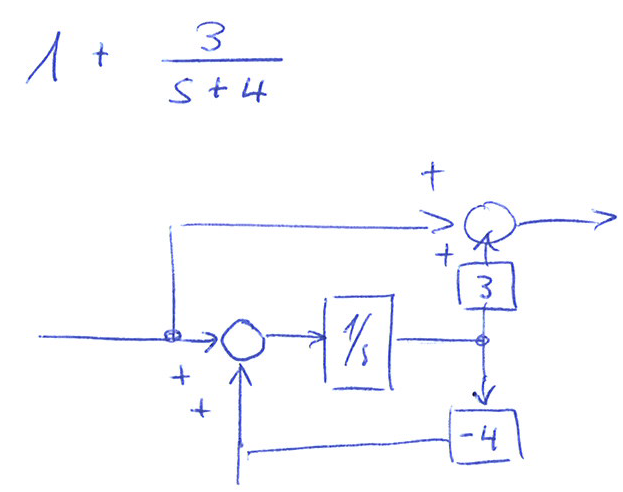
\includegraphics[width=5cm]{./images/implementierung2.png}
%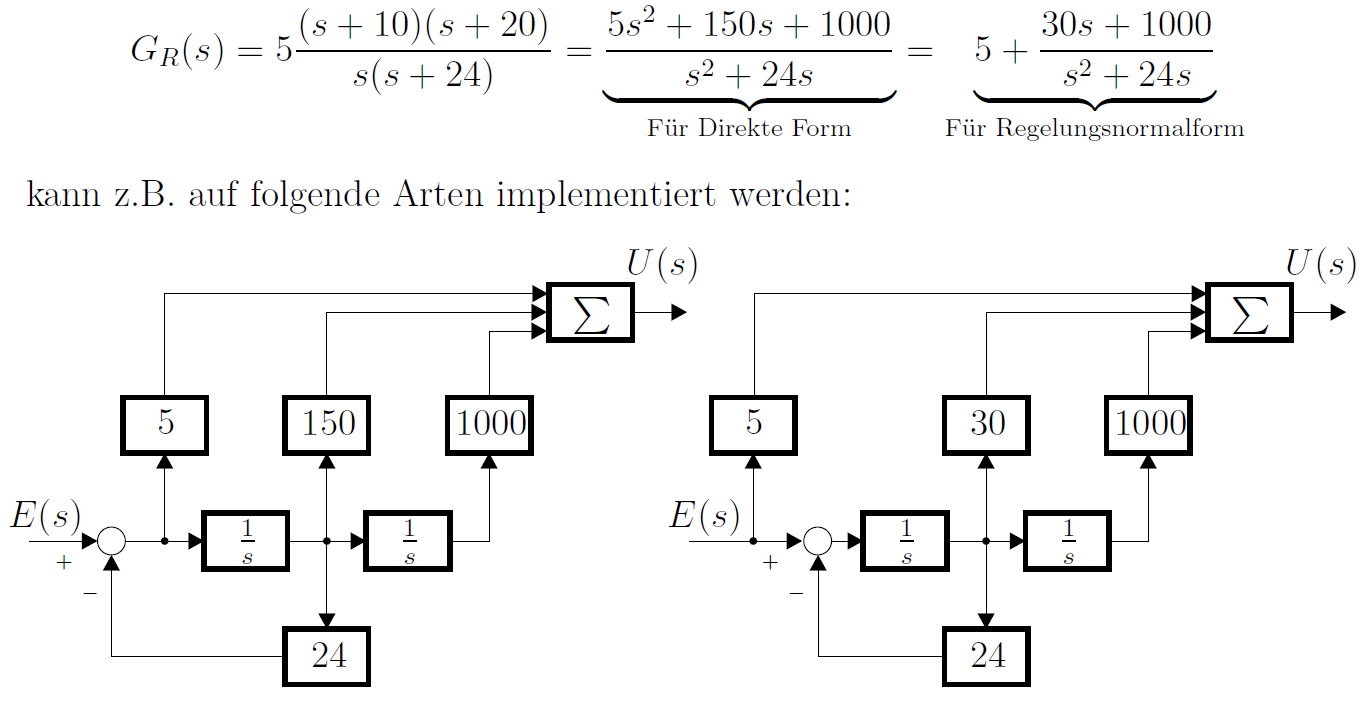
\includegraphics[width=10cm]{./images/implementierung.png}

\begin{center}
	\begin{tabu}{|p{0.25\textwidth}|p{0.7\textwidth}|}
	\hline
	\multicolumn{2}{|c|}{$G(S) = \frac{b_ms^m + b_{m-1}s^{m-1}+\dots + b_1s+b_0}{a_ns^n + a_{n-1}s^{n-1}+\dots + a_1s+a_0} \qquad (m\le n)$}\\[2mm]
	\hline
	\bf{Direkte Form/ Direkte Form II}
		& 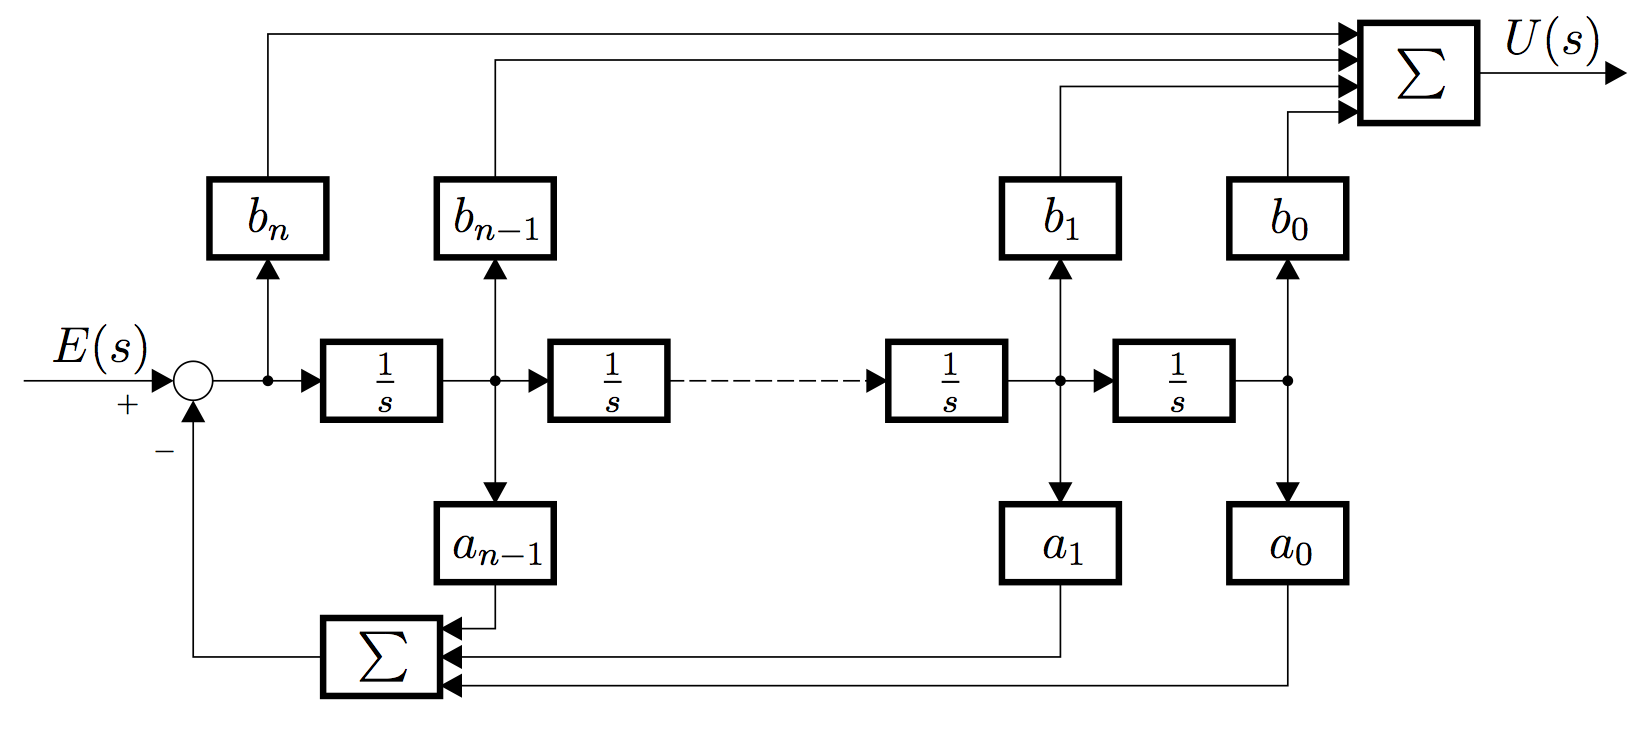
\includegraphics[width = \linewidth, height = 4.2cm, trim = 0 0 0 -5]{./images/DirekteForm2}\\[2mm]
	\hline
	\bf{Transponierte direkte Form/ Direkte Form I}
		& 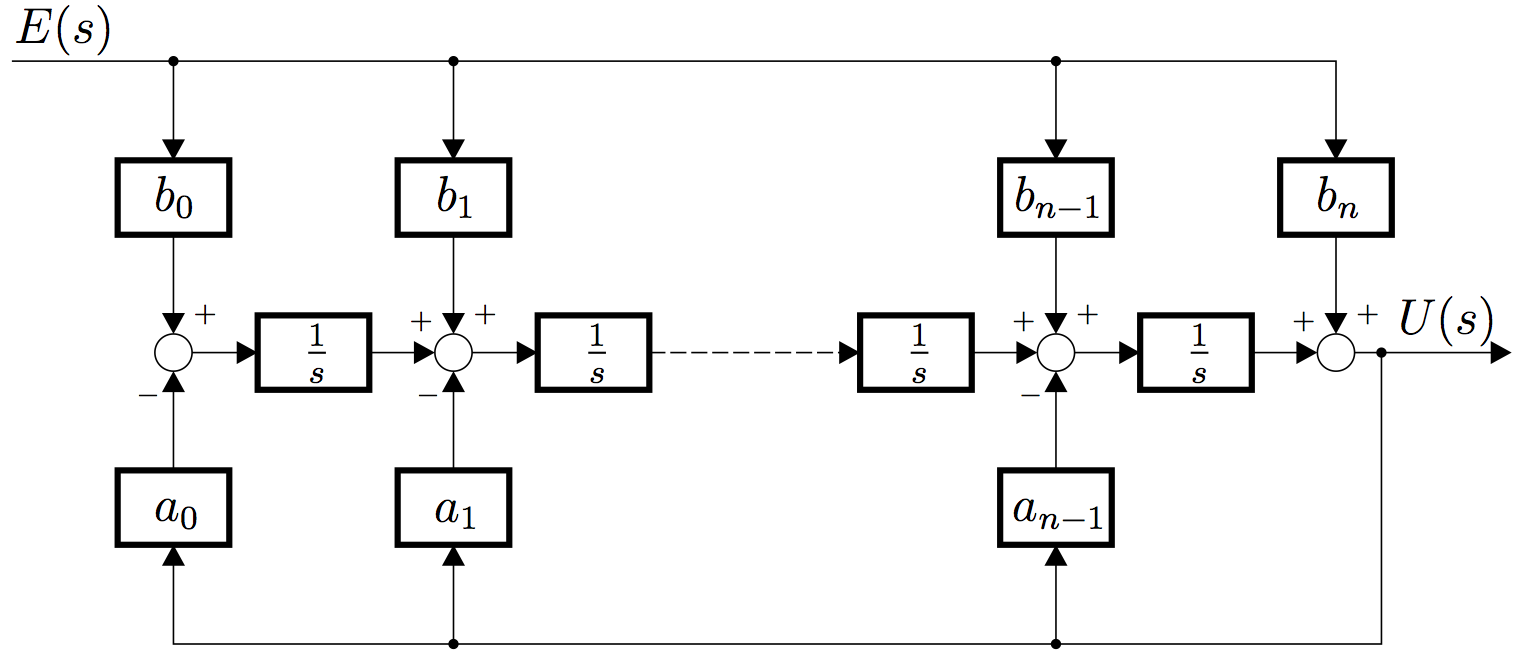
\includegraphics[width = \linewidth, height = 4.2cm, trim = 0 0 0 -5]{./images/DirekteForm1}\\[2mm]
	\hline
	\multicolumn{2}{|c|}{$G(S) = d + \frac{b_ms^m + b_{m-1}s^{m-1}+\dots + b_1s+b_0}{a_ns^n + a_{n-1}s^{n-1}+\dots + a_1s+a_0} \qquad (m < n)$}\\[2mm]
	\hline
	\textbf{Regelungsnormalform}
		& 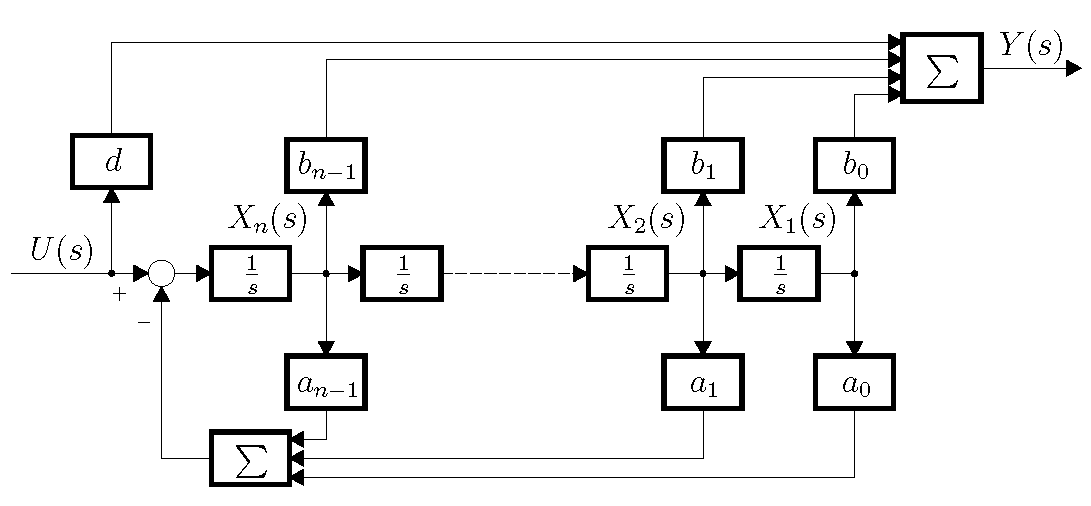
\includegraphics[width = \linewidth, height = 4.2cm, trim = 0 0 0 -5]{./images/regelungsnormalform}\\[2mm]
	\hline
	\end{tabu}
\end{center}
